\chapter{Graphics with TikZ}

There are several methods for producing line graphics in \LaTeX.
We cover here TikZ, which is quite portable across compilers and extremely versatile.
It is contained in the \pkg{tikz} package.
There are several extension libraries that are loaded with the \cmd{usetikzlibrary} command,
and moreover many other packages are built with TikZ.

TikZ has bit of a learning curve
and its documentation spreads over no less than 1321~pages (as of April~2024).
We are able to only cover the essentials here.
An unofficial web version of the manual can be accessed at \url{https://tikz.dev/}.

\begin{technote}
TikZ is an acronym for \emph{TikZ ist kein Zeichenprogramm}
-- ``TikZ is not a drawing program''.
From this we can learn two things:
\begin{itemize}
\item Many \LaTeX{} core developers come from German-speaking Europe.
\item That as useful as TikZ is,
    for complex graphics you probably should use a proper, visual graphics editor.
\end{itemize}
Of course, the the acronym is not only recursive,
but also oxymoronic, since TikZ is a program (written in the \TeX{} language)
that outputs graphics\dots
\end{technote}

\begin{technote}
Internally, TikZ consists of three layers:
compiler-specific support code for primitive drawing operations,
a core layer called PGF,
and the (relatively) user-friendly frontend called TikZ.

Due to this, you can see references to PGF scattered in various places;
for example the CTAN page for \pkg{tikz} redirects to that of \pkg{pgf}.
In practice, the two are synonymous.
\end{technote}


%
%
\section{Coordinates, nodes, and paths}

Let us begin with a very simple example:
%
\begin{VerbatimOut}{\jobname.tmp}
\begin{tikzpicture}
  \draw[->] (0,0) -- (2,0);
  \draw[->] (0,0) -- (0,2);
  \draw[dotted] (0,0) -- ({sqrt(2)}, 1);
\end{tikzpicture}
\end{VerbatimOut}
\ShowExample
%
TikZ pictures are defined inside a \env{tikzpicture} environment.
(For small pictures, there is also a \cmd{tikz} command
that takes the contents of the environment as its single argument.)
The output appears inline in text, just as with \verb|\includegraphics| and friends.

Inside this environment, there are drawing commands.
Each of these commands \emph{ends with a semicolon}.
Forget the \verb|;| and you will get an error message.

The \cmd{draw} command is the basic workhorse of TikZ.
The \verb|--| operation draws a line between the two coordinates.
Let us first look at the syntax of coordinates before going back to the optional arguments
and different operations.

There are several coordinate systems, of which I believe the next four are most common.
\begin{description}
\item[xyz] As in the example above, coordinates in this system are
    tuples or triples of numbers separated by commas.
    These are with respect to unit vectors defined in the environment options.
    By default, the $x$ and $y$ unit vectors are 1~cm long and along the usual axes.
    The $z$ axis is skewed towards the reader.
    See the example on page~\pageref{ex:tikz basis}.

    It is possible to use mathematical syntax like \verb|+|, \verb|/|, and \verb|sqrt(...)|
    to give more complicated coordinate expressions.
    You might need to wrap the calculation inside \verb|{}|.

\item[canvas] The numbers can also have units like \verb|(1cm, 20pt)|.
    In this case the coordinates are the absolute length away from canvas origin.
    It is possible to use expressions like \verb|1cm + 2pt|.
    
    These units are still not completely absolute:
    the canvas can still be scaled with an optional argument.

    \emph{Warning}: While it is technically possible to mix canvas and xyz coordinates
    inside the tuple, it is ill-advised.
    Similarly, an expression like \verb|1+2cm| is interpreted as \verb|1pt+2cm|,
    not as ``unit vector plus 1~cm to the right''.

\item[xyz polar] Polar coordinates are like \verb|(30:2)|,
    which means: 30 degrees counterclockwise, radius 2~units.

    If the $x$ and $y$ unit vectors are set to non-default values,
    the angle corresponds to a point on the ellipse specified by $x$ and $y$ vectors,
    and the resulting vector is multiplied by the radius factor.

\item[canvas polar] Here the radius has a specified unit: \verb|(30:2cm)|.
\end{description}

There are also the barycentric coordinate system (weighted average of basis vectors)
and a possibility to compute tangents of shapes.
These are covered in \cite[Section~13.2]{tikz}.

Coordinates can be given names with the \cmd{coordinate} command.
In the example below, we also use the \verb|cycle| specifier to close the loop.
%
\begin{VerbatimOut}{\jobname.tmp}
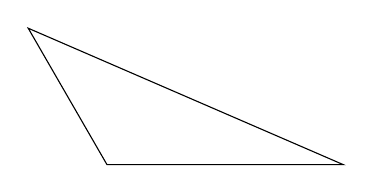
\begin{tikzpicture}
  \coordinate (A) at (0:3cm);
  \coordinate (B) at (120:2cm);

  \draw (0,0) -- (A) -- (B) -- cycle;
\end{tikzpicture}
\end{VerbatimOut}
\ShowExample

It is also possible to specify relative coordinates:
by prefixing the coordinate with \verb|++|, it is relative to the previous position.%
\footnote{It is also possible to prefix with just \texttt{+},
in which case the current position is not updated.}
%
\begin{VerbatimOut}{\jobname.tmp}
\begin{tikzpicture}
  \draw (0,0) -- ++(0:3) -- ++(90:2)
    -- ++(180:1) -- ++(270:1/2);
\end{tikzpicture}
\end{VerbatimOut}
\ShowExample


%
%
\subsection{Nodes}

Nodes can be thought of as text placed in the picture.
The text can contain mathematics and formatting commands, and even pictures.

A node can be placed either as part of a path, or separately with a \cmd{node} command.
In the latter case, it is possible to refer to the node later.
%
\begin{VerbatimOut}{\jobname.tmp}
\begin{tikzpicture}
  \draw (0,0) -- (2,0) node {Left};
  \node (A) at (0,2) {Above};
  \draw (0,0) -- (A);
  \node at (0,-1) {Below};
\end{tikzpicture}
\end{VerbatimOut}
\ShowExample

Note the difference between the lines connecting the origin to the Left and Above nodes.
When a node is created as part of a path operation,
it is \emph{centered} at the specified coordinate.
That is, the center of the ``Left'' text is at $(2,0)$.
The position of the node can be customized by passing
\verb|above|, \verb|below|, \verb|left|, or \verb|right| as an optional argument.

On the other hand, when a path is drawn to a previously defined node,
TikZ tries to stop at the boundary of the node.
It is possible to specify the position on the border by cardinal directions (like \verb|north|)
or an angle; or to specify \verb|center| if you really mean the center.
These are given by the \verb|name.anchor| syntax as in the example below.

To make the boundary of the ``Above'' node visible,
we also pass the \verb|draw| option to the \cmd{node} command.
%
\begin{VerbatimOut}{\jobname.tmp}
\begin{tikzpicture}
  \draw (0,0) -- (2,0) node[right] {Left};
  \node[draw] (A) at (0,2) {Above};
  \draw (0,0) -- (A.west);
\end{tikzpicture}
\end{VerbatimOut}
\ShowExample

One more interesting positioning specifier is the optional \verb|pos| argument.
It is understood as a position (in the range 0 to 1) on the previous path segment.
It can be combined with other specifiers as in here:
%
\begin{VerbatimOut}{\jobname.tmp}
\begin{tikzpicture}
  \draw[->] (0,0) -- (3,0)
    node[pos=0.5,above] {$\frac 1 2$}
    node[pos=0.25,below] {$\frac 1 4$}
    node[pos=0.75,below] {$\frac 3 4$};
\end{tikzpicture}
\end{VerbatimOut}
\ShowExample

To embed pictures,
you can use \cmd[in TikZ]{includegraphics} as usual inside a node.
To illustrate this once more with our fur-shedding assistants:
%
\begin{VerbatimOut}{\jobname.tmp}
\centering
\newcommand{\dogfile}{pictures/TheDogs.jpg}
\begin{tikzpicture}
  \node[draw] (Both) at (0,0)
    {\includegraphics[height=3cm]{\dogfile}};
  \node[draw] (Netta) at (-5,0)
    {\includegraphics[bb=1cm 2cm 3cm 5cm, clip, height=2cm]{\dogfile}};
  \node[draw] (Cira) at (5,0)
    {\includegraphics[bb=2.8cm 1.4cm 7cm 6cm, clip, height=2cm]{\dogfile}};
  \draw[->] (Both.west) -- (Netta.east) node[pos=0.5, above] {Netta};
  \draw[->] (Both.east) -- (Cira.west) node[pos=0.5, above] {Cira};
\end{tikzpicture}
\end{VerbatimOut}
\ShowExampleBelow[2]


%
%
\subsection{Path options}

There are lots of options that can be passed to the drawing commands.
As the very first one, let us consider \verb|color|.
It takes a colour name as its argument;
\pkg[with TikZ]{xcolor} extensions and custom colours are supported.
It is possible to blend the color with white with the \verb|!| specifier
(see page~\pageref{ex:color blending}).
Be careful with the colour name; the error message can be confusing.
%
\begin{VerbatimOut}{\jobname.tmp}
\definecolor{Sciency}{cmyk}{0,0.46,1,0}
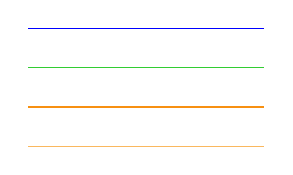
\begin{tikzpicture}
  \draw[color=blue] (0,0)--++(3,0);
  \draw[color=LimeGreen] (0,-0.5)--++(3,0);
  \draw[color=Sciency] (0,-1)--++(3,0);
  \draw[color=Sciency!60] (0,-1.5)--++(3,0);
\end{tikzpicture}
\end{VerbatimOut}
\ShowExample

There is also a range of line weights.
Do note that their names may include spaces.
Of these, \verb|thin| is the default.
%
\begin{VerbatimOut}{\jobname.tmp}

\begin{tikzpicture}[yscale=0.8]
  \draw[very thin] (0,-0.5)--++(3,0);
  \draw[thin] (0,-1)--++(3,0);
  \draw[semithick] (0,-1.5)--++(3,0);
  \draw[thick] (0,-2)--++(3,0);
  \draw[very thick] (0,-2.5)--++(3,0);
  \draw[ultra thick] (0,-3)--++(3,0);
\end{tikzpicture}
\end{VerbatimOut}
\ShowExample

Then, there are the line styles.
The basic ones are (it is possible to specify custom ones, but that you have to read from the docs):
%
\begin{VerbatimOut}{\jobname.tmp}
\begin{tikzpicture}[yscale=0.8]
  \draw[solid] (0,0.5)--++(3,0);
  \draw[dashed] (0,-0)--++(3,0);
  \draw[dotted] (0,-0.5)--++(3,0);
  \draw[densely dashed] (0,-1)--++(3,0);
  \draw[densely dotted] (0,-1.5)--++(3,0);
  \draw[loosely dashed] (0,-2)--++(3,0);
  \draw[loosely dotted] (0,-2.5)--++(3,0);
  \draw[dash dot] (0,-3)--++(3,0);
  \draw[dash dot dot] (0,-3.5)--++(3,0);
\end{tikzpicture}
\end{VerbatimOut}
\ShowExample

\begin{practices}
As remarked in the section on colour,
you should never use colour as the sole means of giving information.
In simple line graphics, the combination of colour and line style is often useful.
However, complex line styles are also hard to read!
\end{practices}


Finally, there are the arrows.
The syntax for arrow tips is $\langle\textit{start}\rangle$\verb|-|$\langle\textit{end}\rangle$,
where the start/end specification can contain one or more \verb|<|, \verb|>|, or \verb$|$.
%
\begin{VerbatimOut}{\jobname.tmp}
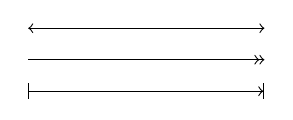
\begin{tikzpicture}[yscale=0.8]
  \draw[<->] (0,-0)--++(3,0);
  \draw[->>] (0,-0.5)--++(3,0);
  \draw[|->|] (0,-1.0)--++(3,0);
\end{tikzpicture}
\end{VerbatimOut}
\ShowExample
%
The \verb|arrows.meta| extension library contains many more tip styles
and options to customize their size; see \cite[Section~16]{tikz}.
%
\begin{VerbatimOut}{\jobname.tmp}
% \usetikzlibrary{arrows.meta}
\begin{tikzpicture}[yscale=0.8]
  \draw[Circle-{Circle[open]}] (0,-0)--++(3,0);
  \draw[-{Stealth[length=5mm,width=2mm,red]}] (4,0)--++(3,0);
  \draw[{->[harpoon]}] (8,0)--++(3,0);
\end{tikzpicture}
\end{VerbatimOut}
\ShowExampleBelow

One more option: the \verb|rounded corners| option does what is says.
It takes as its argument a radius of the corner.
It is one of the few options that can be changed in the middle of a path
(none of the above can, unfortunately).
%
\begin{VerbatimOut}{\jobname.tmp}
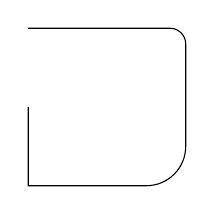
\begin{tikzpicture}
  \draw[rounded corners=2mm] (0,0) -- (2,0)
    [rounded corners=5mm] -- (2,-2)
    [sharp corners] -- (0,-2) -- (0,-1);
\end{tikzpicture}
\end{VerbatimOut}
\ShowExample



%
%
%
\section{Special paths}

In addition to the \verb|--| style path joining two points,
there are the \verb$|-$ and \verb$-|$ styles.
These split the line into vertical and horizontal segments,
the order of which you can probably guess.
%
\begin{VerbatimOut}{\jobname.tmp}
\begin{tikzpicture}
  \draw (0,0) -| (2,1);
\end{tikzpicture}
\end{VerbatimOut}
\ShowExample

To draw rectangles, there is the \verb|rectangle| shorthand
that is put between coordinates of the two opposite corners.
Similarly, there is the \verb|circle| command that is put after the centre coordinate
and takes the radius as an optional parameter.
It is possible to specify \verb|x radius| and \verb|y radius| separately to get an ellipse
(which can be further rotated with the \verb|rotate| parameter).
%
\begin{VerbatimOut}{\jobname.tmp}
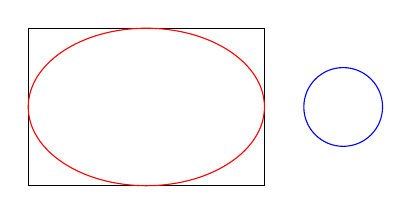
\begin{tikzpicture}
  \draw (0,0) rectangle (3,2);
  \draw[red] (3/2,1) circle
    [x radius=3/2, y radius=1];
  \draw[blue] (4,1) circle [radius=0.5];
\end{tikzpicture}
\end{VerbatimOut}
\ShowExample

There are also commands for drawing arcs, parabolas, and even Bézier curves;
see \cite[Section~14]{tikz}.

There is a helper command for drawing coordinate grids.
TikZ provides a shorthand style \verb|help lines|
that can be customized as in \Cref{sec:tikz styles}.
Here we overlay two grids with different step sizes (default is one unit).
%
\begin{VerbatimOut}{\jobname.tmp}
\centering
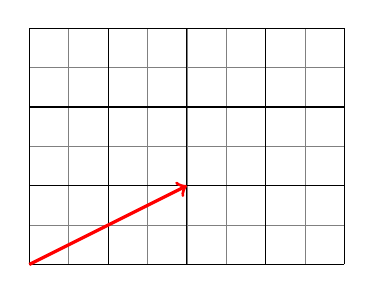
\begin{tikzpicture}
  \draw[help lines, xstep=0.5, ystep=0.5] (0,0) grid (4,3);
  \draw (0,0) grid (4,3);
  \draw[red,very thick,->] (0,0) -- (2,1);
\end{tikzpicture}
\end{VerbatimOut}
\ShowExampleBelow[2]

Now that we know how to draw a coordinate grid,
it is very natural to draw some functions on it!
TikZ includes a reasonably complex calculation engine,
which makes it possible to draw some complicated functions.
%
\begin{VerbatimOut}{\jobname.tmp}
\centering
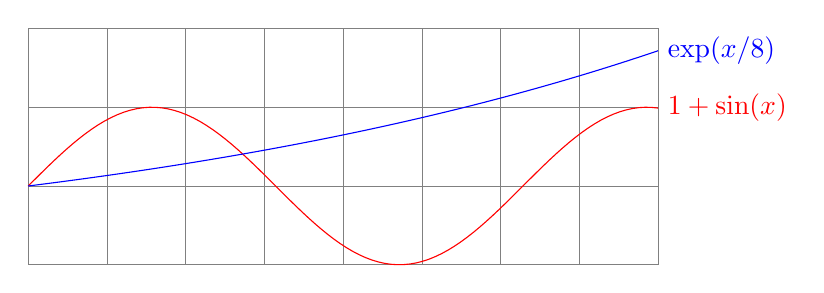
\begin{tikzpicture}
  \draw[help lines] (0,0) grid (8,3);
  \draw[red, domain=0:8, samples=100] plot (\x, {1+sin(\x r)})
    node[right] {$1+\sin(x)$};
  \draw[blue, domain=0:8, samples=100] plot (\x, {exp(\x/8)})
    node[right] {$\exp(x/8)$};
\end{tikzpicture}
\end{VerbatimOut}
\ShowExampleBelow[2]
Some notes on the usage:
\begin{itemize}
\item The domain is specified using the syntax \verb|lower:upper|.
\item The number of samples is optional to specify, but the default value is quite small.
\item The variable $x$ is written with a backslash \verb|\x|,
    but the mathematical commands are spelled without a backslash.
\item Mathematical expressions should be wrapped inside \verb|{}|.
\item Trigonometric functions assume degrees by default;
    the suffix \verb|r| after \verb|\x| converts the variable into radians.
\end{itemize}

Note that the plot is still defined as a pair of $(x,y)$ coordinates.
This makes it possible to draw parametric plots.
The name of the variable can be customized.
%
\begin{VerbatimOut}{\jobname.tmp}
\centering
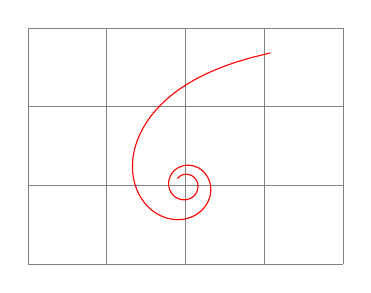
\begin{tikzpicture}
  \draw[help lines] (-2,-1) grid (2,2);
  \draw[red, domain=1:15, samples=150, variable=\t]
    plot ({2*cos(\t r) / \t}, {2*sin(\t r) / \t});
\end{tikzpicture}
\end{VerbatimOut}
\ShowExampleBelow[2]

It is also possible to plot individual points or bar graphs,
or to even load a dataset from an external file.
See \cite[Section~22]{tikz} for more,
but also note the warnings below.

\begin{warning}
``Division by zero'' and ``number too big`` errors
can sometimes lead to confusing (and repeated!) error messages.
\end{warning}

\begin{practices}
TikZ is excellent for producing small and simple function plots
in a style consistent with the rest of the document.
However, compilation times can get quite long for even slightly complicated functions.

I would therefore not recommend using TikZ for complex graphics.
If you still need it, consider disabling the plots in \verb|draft| mode
(by some conditional evaluation; see \Cref{sec:if}).
\end{practices}



%
%
\section{Transformations}

\todo{useasboundingbox}


%
%
\section{Loops}


%
%
\section{Setting styles}\label{sec:tikz styles}


%
%
\section{Some extensions}

\todo{Think about what to cover here: angles, decorations, graphs, trees, spy?}
